\section{Cloud Caching}

FlyingSquid leverages different cloud storage tiers, each with unique benefits, to build a more sophisticated caching infrastructure. As a result, individual instances in an ATS cluster can be configured to share access to cached objects and use storage space more efficiently.

\begin{figure}[H] \centering
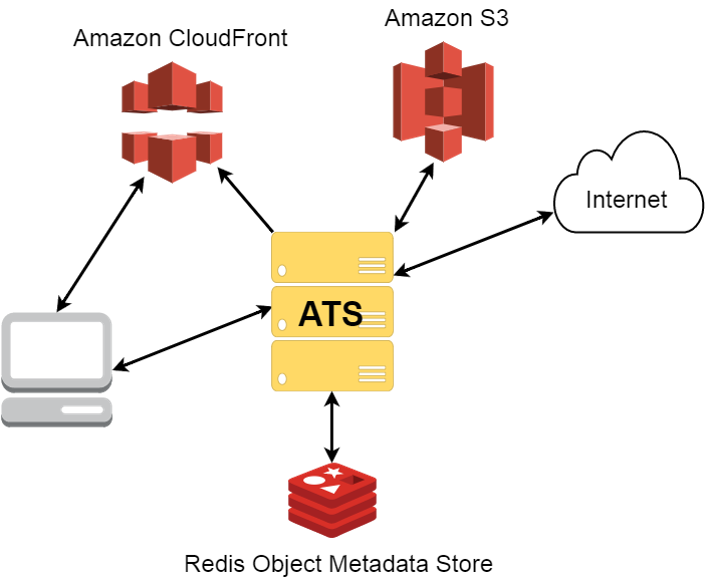
\includegraphics[width=\textwidth]{CloudCachingArch}
\caption{Flying Squid Proxy Cloud Caching Architecture}
\end{figure}

\subsection{Augmented Tier - Redis Cluster}
FlyingSquid uses a Redis in-memory key/value store to save HTTP object metadata. Each member of an ATS cluster has a master and slave pair of Redis instances. These instances are connected as a cluster and objects are stored across these instances according to how the cluster partitions keys. We chose to use this storage format for object metadata as opposed to storing data with each object because we needed a faster method of accessing data than querying S3 (where all cache objects are ultimately stored), as this type of query will inherently introduce significant performance penalties.

\newpage

\noindent
FlyingSquid uses the ATS computed cache key hash for each object as the key to store metatadata under and serialize the struct below to a string to store it in Redis.

\begin{lstlisting}
struct ObjectCacheMeta {
    int64_t size; // Object size in bytes
    int64_t headerLength;
    char *responseHeader; // Response header to send back to client
    long lastAccessed; // Unix timestamp of when object was last accessed
    long cloudFrontExpiry; // Unix timestamp of when object will be removed from CloudFront
  };
\end{lstlisting}

\noindent
Whenever we do a cache write we insert or update this object metadata. When we do cache reads and access objects in the cache, we update the lastAccessed timestamp and if applicable update the cloudFrontExpiry field.

\subsection{Storage Tier - AWS Simple Storage Service (S3)}
FlyingSquid utilizes Amazon S3 public cloud storage as the largest and slowest tier of the cloud cache. An ATS cluster is configured to share storage of HTTP objects in a S3 bucket. When ATS determines that an HTTP object is cacheable the object is uploaded to S3. When a cache read is called for we determine whether an object is in S3 from the Redis object metadata. If so, we simply retrieve it, collect the header from Redis, and send it back to the client.

\subsection{Storage Tier - AWS Cloudfront}

